\subsection{Progettazione Architetturale}
Periodo: dal 2020-01-22 al 2020-03-15\\
Inizia al termine della fase di Analisi e finisce con la data di consegna per la Revisione di Progettazione.\\
In questa fase viene definita una soluzione architetturale in modo da soddisfare i requisiti individuati nella fase di Analisi.

\subsubsection{Periodo 1} 
Dal 2020-01-22 al 2020-02-20
\begin{itemize}
	\item \textbf{Normazione}: Standardizzazione e correzione di alcune parti della documentazione che non aderiscono completamente alle \NdP{};
	\item \textbf{\AdR{}}: Avvio della correzione e modifica dei casi d'uso segnalati, concentrandosi sui casi d'uso e requisiti segnalati (e non) utili al PoC;
	\item \textbf{Assegnazione dei ruoli di progetto}: Assegnazione dei ruoli di ciascun membro del gruppo in base alla suddivisione oraria indicata in §5.2.1;
	\item \textbf{Pianificazione delle attività}: Le attività da svolgere devono essere prima pianificate e discusse dal gruppo per garantire il \glo{way of working} sancito nelle \NdP{};
	\item \textbf{Approfondimento e studio delle tecnologie}: Ricerca di documentazione e materiali utili per l'apprendimento delle nuove tecnologie da utilizzare per la realizzazione del prodotto finale.
	In particolare:
	\begin{itemize}
		\item per l'app per gli utenti: Java per Android, l'IDE Android Studio, le API di Google per Google Maps, Firebase, Google Play, il formato JSON, la libreria client HTTP Volley;
		\item per la web app per gli amministratori: il tool di build automation Node.js, i framework Angular e Bootstrap, TypeScript;
		\item per il server: il tool di build automation Maven e i suoi plugin, gli strumenti di Swagger e lo standard OpenAPI, il framework Spring per Java, il database Redis.
	\end{itemize}
	\item \textbf{Verifica}: \glo{Verifica} dell'andamento del team in relazione alle tempistiche e allo svolgimento dei compiti assegnati.
\end{itemize}

\subsubsection{Periodo 2} 
Dal 2020-02-17 al 2020-03-08
\begin{itemize}
	\item \textbf{Studio delle tecnologie}: l'\glo{IaaS} \glo{Kubernetes} o i \glo{PaaS} \glo{Openshift} o \glo{Rancher}, \glo{LDAP}, \glo{GPS} e Android Studio;
	\item \textbf{Normazione}: Decisioni ed inserimento delle nuove regole da adottare per le attività di progettazione e sviluppo;
	\item \textbf{Miglioramento standard di qualità}: Aggiunta, rimozione o modifica di alcune metriche per garantire le qualità di \glo{processo} e di prodotto affermate nel \PdQ{};
	\item \textbf{Incrementi}: Per facilitare l'organizzazione del lavoro di progettazione e di implementazione, vengono indicati qui di seguito gli incrementi che vengono portati avanti (come indicato in §3.3):
		\begin{itemize}
			\item \textbf{Incremento 1}: Vengono progettate e successivamente implementate le funzionalità di \glo{autenticazione} per l'utente e per l'amministratore;
			\item \textbf{Incremento 2}: Vengono progettate e successivamente implementate la gestione delle liste delle \glo{organizzazioni} dell'applicazione e del server;
			\item \textbf{Incremento 3}: Vengono progettate e successivamente implementate la gestione delle \glo{modalità} di tracciamento;
			\item \textbf{Incremento 4}: Viene progettato e successivamente implementato lo storico degli accessi di un utente nell'applicazione e il report tabellare degli accessi nel server;
			\item \textbf{Incremento 5}: Viene progettata e successivamente implementata l'autenticazione presso l'organizzazione nell'applicazione e la modifica dell'organizzazione nel server;
			\item \textbf{Incremento 6}: Viene progettata e successivamente implementata la gestione degli amministratori nel server.
		\end{itemize}
		L'obiettivo è progettare almeno i requisiti obbligatori degli incrementi e avere un \glo{Proof of Concept} che li sappia dimostrare correttamente, in modo da avere una solida \glo{baseline} per le successive fasi;
	\item \textbf{Progettazione}: Ricerca di una soluzione soddisfacente per tutti gli \glo{stakeholder}, che descriva l'architettura del prodotto prima di pensare al codice, seguendo gli incrementi definiti;
	\item \textbf{Technology Baseline}: Redazione della \glo{Technology Baseline}, cioè un allegato tecnico nel quale vengono indicate le tecnologie e i design pattern che vengono utilizzati durante lo sviluppo del prodotto;
	\item \textbf{Proof of Concept}: Creazione di un eseguibile che permetta di dimostrare la validità del prodotto che si vuole fornire, concretizzando la \glo{Technology Baseline};
	\item \textbf{Codifica}: Viene codificato il \glo{Proof of Concept} e successivamente condiviso tramite i \glo{repository} del gruppo al committente e al proponente in una data da definire;
	\item \textbf{Verifica}: \glo{Verifica} dell'andamento del gruppo in relazione alle tempistiche e allo svolgimento dei compiti assegnati.
\end{itemize}

\subsubsection{Periodo 3} 
Dal 2020-03-09 al 2020-03-15
\begin{itemize}
	\item \textbf{Consolidamento}: Ogni membro si prende del tempo per ripassare tutto il lavoro svolto e per studiare il necessario per affrontare al meglio le fasi successive;
	\item \textbf{Preparazione per la Revisione di Progettazione}: Il gruppo produce il materiale necessario da esporre alla presentazione pubblica della propria proposta.
\end{itemize}


\newpage
% Inizia la pagina orientata orizzontalmente
\begin{landscape}
% Ora la pagina e' in orizzontale!
\subsubsection{Diagramma di Gantt delle attività della fase di Progettazione Architetturale}
\pagestyle{empty}
\begin{figure}[h]
	\centering
	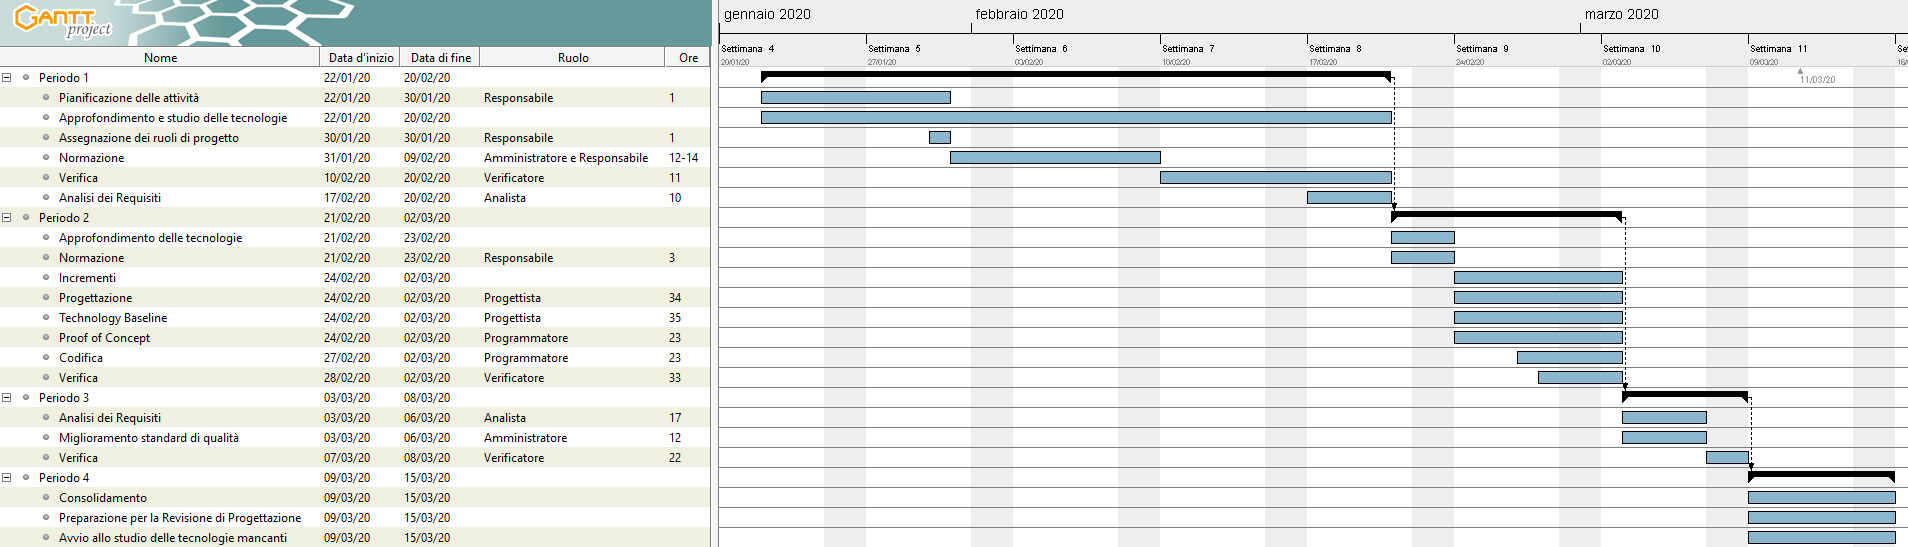
\includegraphics[scale=0.34]{Sezioni/DiagrammiGantt/ProgettazioneArchitetturale.png}
	\caption{Diagramma di Gantt delle attività della fase di Progettazione Architetturale}	
\end{figure}
\end{landscape}
\clearpage